% !TeX root = ../main.tex

% Document-wide defines
\newcommand{\Reals}{{\rm I\!R}}

% DEVS model definition helpers
\newcommand{\deltaInt}[1]{
    \begin{algorithm}[H]
        \caption{$\delta_{int} (s)$}
        \begin{algorithmic}
        #1
        \end{algorithmic}
    \end{algorithm}
}
\newcommand{\deltaExt}[1]{
    \begin{algorithm}[H]
        \caption{$\delta_{ext} (s,e,x)$}
        \begin{algorithmic}
        #1
        \end{algorithmic}
    \end{algorithm}
}
\newcommand{\lambdaOut}[1]{
    \begin{algorithm}[H]
        \caption{$\lambda (s)$}
        \begin{algorithmic}
        #1
        \end{algorithmic}
    \end{algorithm}
}

\section{Especificación Formal}

\subsection{Modelos Atómicos}

\subsubsection{Panel solar y generador eólico}
Como fue descripto en el modelo conceptual (\ref{section:modeloConceptual}),
el modelo que representa al panel solar, y también al generador eólico son
simples. Ambos tendrán un puerto de entrada, el cual recibirá el valor de la
magnitud de clima que los afecta, siendo radiación en el caso del primero, y
la velocidad del viento para el segundo. Por otro lado, tendrán un puerto de
salida, por el cual notificarán a los modelos que tengan una conexión al
mismo, cual es la nueva cantidad de energía que están produciendo.

% TODO: Poner algo haciendo referencia a que DEVS puede manejar eventos (cambios en dichas magnitudes climáticas) a distintas frecuencias de ocurrencia. Leer en el Wainer como se explicaba esto.
% TODO: Poner las funciones de transición, y las funciones matemáticas con las cuales se calculará la potencia producida.

$Generador = <X,Y,S,\delta_{int}, \delta_{ext}, \lambda, ta>$

Definiendo cada elemento de la tupla DEVS como:

\begin{align*}
X &= \Reals_{\geq0} & Y &= \Reals_{\geq0} & S &= energiaProducida \in \Reals_{\geq 0} \\
\end{align*}

\deltaInt{
    \STATE passivate()
}

\deltaExt{
    \STATE $energiaProducida \leftarrow calcularPotenciaProducida(x.value) $
}

\lambdaOut{
    \STATE sendOutput(time, out, energiaProducida)
}

\subsubsection{Batería}
El modelo de la batería consta de tres puertos de entrada y dos de salida.

Tiene un puerto en el cual recibe los cambios en la cantidad de energía generada
por el generador eólico y otro en el cual recibe la generada por el panel solar.
En el tercer puerto recibe la cantidad de energía solicitada por el controlador.

Los puertos de salida son el del estado de la batería, que informa el estado actual
de la batería, que puede ser:

\begin{itemize}
    \item \emph{Vacía}: En este estado, la carga es 0, y se mantiene en él, hasta
        que llegue energía por alguno de los generadores.
    \item \emph{Cargando}: Posee carga, pero se encuentra por debajo del límite
        mínimo para enviar. En este estado, la batería no hace disponible la carga.
    \item \emph{Disponibe}: En este estado, la batería ya se encuentra disponible
        para enviar carga, pero aún no esta llena.
    \item \emph{Completa}: Ocurre cuando la carga alcanza la máxima capacidad. En este
        estado, la batería informa al controlador la cantidad de energía que se está
        produciendo en exceso, para que pueda entregarla a la red.
\end{itemize}

Hay que aclarar que la batería no pasa del estado \emph{Disponibe} al \emph{Cargando}
cuando se consume la carga y esta alcanza niveles por debajo del limite de envío, sino que
la batería continúa enviando hasta que pasa al estado \emph{Vacía}.

Así, el conjunto de variables que conforman de estado de la batería, es el siguiente:

\begin{itemize}
    \item \textbf{solarPanelPower:} Cantidad de energía enviada desde el panel solar.  Real mayor o igual a 0.
    \item \textbf{windTurbinePower:} Cantidad de energía enviada desde la turbina eolica.  Real mayor o igual a 0.
    \item \textbf{controllerDemand:} Cantidad de energía solicitada por el controlador. Real mayor o igual a 0.
    \item \textbf{charge:} Energía acumulada en la batería. Real mayor o igual a 0
    \item \textbf{lastChargeUpdate:} Tiempo en que se realizó la ultima actualización del estado de la carga.
    Variable de tipo VTime, mayor a 0
    \item \textbf{state:} Estado actual de la batería. Uno de los cuatro valores mensionados anteriormente.
\end{itemize}

Formalmente, $S \in \mathbb{R}_{\geq 0}^4 \times VTime_{\geq 0} \times \{Vacia, Cargando, Disponibe, Completa\}$ 

Para calcular el valor real de la carga que posee la batería en el tiempo actual $t$, 
tenemos que combinar todas estas variables de estado:

$$CargaReal = charge+(lastChargeUpdate - t) \times \Delta_{energia}$$

Donde $\Delta_{energia}$ es igual a la diferencia de la energía producida por los generadores y la enviada
por la batería.

Con cada cambio de alguna de estas variables, actualizamos el valor de \textbf{charge} para así
mantener la ecuación descripta anteriormente.

Esta misma formula se puede reescribir para calcular cuando sucederá el próximo cambio de la variable $state$:

$$ta = \frac{CargaEnProximoEstado - charge}{\Delta_{energia}}$$

En cuanto a las transiciones externas, en ellas tenemos que recalcular \textbf{charge} y el momento en que se
producirá el proximo cambio de estado.

\deltaExt{
    \STATE {charge $\leftarrow$ calculate\_current\_charge(s, e)}
    \IF {x.port = SOLAR\_PANEL}
        \STATE S' $\leftarrow$ $<$x.value, S.windTurbinePower, S.controllerDemand, charge, e, s.state$>$
    \ELSIF{x.port = EOLIC\_TURBINE}
        \STATE S' $\leftarrow$ $<$S.solarPanelPower, x.value, S.controllerDemand, charge, e, s.state$>$
    \ELSIF{x.port = REQUIRED\_ENERGY}
        \STATE S' $\leftarrow$ $<$S.solarPanelPower, S.windTurbinePower, x.value, charge, e, s.state$>$
    \ENDIF
    \STATE next\_change $\leftarrow$ calculate\_next\_event(S')
    \RETURN {S'}
}

Las transiciones internas, se corresponden a cambios en del estado.

\lambdaOut{
    \STATE {charge $\leftarrow$ calculate\_current\_charge(s, current\_time)}
    \STATE {(S', next\_change) $\leftarrow$ calculate\_next\_state(s, charge, current\_time)}
    \RETURN {S'}
}

\lambdaOut{
    \STATE {charge $\leftarrow$ calculate\_current\_charge(s, current\_time)}
    \STATE {(S', next\_change) $\leftarrow$ calculate\_next\_state(s, charge, current\_time)}
    \STATE {sendOutput(time, battery\_state\_port, S'.state)}
    \IF {S'.state = \emph{Completa}}
        \STATE {sendOutput(time, out, $\Delta_{energy}$(S'))}
    \ENDIF
}

Hay que mencionar que, si bien no se refleja en el pseudocódigo, también usamos las
transiciones internas para poder informar cambios en la cantidad de energía sobrante cuando
la batería se encuentra llena, ya que si bien no cambia el valor de la variable \textbf{state},
no podemos hacer uso de la función de output desde transiciones externas.

\subsubsection{Controlador}

El modelo del controlador consta de seis puertos, tres de entrada y tres de salida.

Uno de los puertos de entrada es donde recibe las solicitudes de la carga, otro
es donde recibe el estado actual de la batería y el tercero es por donde la batería 
le avisa la cantidad de energía sobrante.

En cuanto a los puertos de salida, uno de ellos se corresponde a los pedidos de 
energía que hace a la red, otro a los que hace a la batería y el tercero a la cantidad de 
energía que se vende a la red.

En cuanto al estado interno del controlador, el mismo debe almacenar los siguientes valores:

\begin{itemize}
    \item \textbf{batteryState:} Almacena el estado actual de la batería que tiene conectada,
    es necesario para determinar si podemos pedirle energía a la misma o no.
    \item \textbf{currentLoadDemand:} Cantidad de energía solicitada por la carga.
    \item \textbf{batteryDemand:} Cantidad de energía solicitada a la batería.
    \item \textbf{gridDemand:} Cantidad de energía solicitada a la red.
    \item \textbf{extraEnergy:} Cantidad de energía sobrante, informada por la batería.
    \item \textbf{state:} Puede ser \emph{AllGrid} o \emph{GridAndBattery}. En el primer
        caso, toda la energía se está pidiendo a la red, mientras que en el segundo, se
        le pide a la batería, y todo aquello que esté por encima de la máxima potencia
        de salida de la batería, se lo pide a la red.
\end{itemize}

También forman parte del estado las variables \textbf{notifyBattery} y \textbf{notifyExtraEnergy}
cuyo objetivo es poder simular el envío de mensajes en transiciones externas a través del envío
en transiciones internas agendadas a tiempo 0, luego que las externas.

El modelo actual tiene el siguiente comportamiento: Si la batería esta disponible, le solicitará
toda la carga necesaria para cubrir las necesidades de la carga, siempre que esta no supere
el umbral definido, en cuyo caso le pedirá el máximo posible y lo demás lo pedirá de la red.
Si la batería está descargada, esta dejará de suministrarle energía hasta que no se encuentre
disponible nuevamente.

En el caso de que la batería le informe que tiene un excedente de producción, el controlador
lo enviará a la red.

% TODO: Update all function below
\deltaExt{
    \STATE S' $\rightarrow$ S
    \IF {x.port = batterySurplusEnergy}
        \STATE S'.notifyExtraEnergy $\rightarrow$ \textbf{true}
        \STATE S'.extraEnergy $\leftarrow$ x.value
        \RETURN S'
    \ELSIF {x.port = batteryStatePort}
        \STATE S'.batteryState $\leftarrow$ x.value
        \STATE S' $\leftarrow$ updateControllerState(S')
    \ELSIF {x.port = loadDemand}
        \STATE S'.loadDemand $\leftarrow$ x.value
    \ENDIF
    \STATE S' $\leftarrow$ UpdateGridConsuption(S')
    \STATE nextChange = 0
    \RETURN S''
}

\begin{algorithm}
    \caption{$updateControllerState(S)$}
    \begin{algorithmic}[H]
        \STATE S' $\leftarrow$ S
        \IF {S.batteryState = AVAILABE and S.state = AllGrid}
            \STATE S'.state $\leftarrow$ GridAndBattery
        \ELSIF {S.batteryState = EMPTY and S.state = GridAndBattery}
            \STATE S'.state $\leftarrow$ AllGrid
            \STATE S'.notifyBattery $\leftarrow$ \textbf{true}
        \ENDIF
        \RETURN S'
    \end{algorithmic}
\end{algorithm}

\begin{algorithm}
    \caption{$updateGridConsuption(S)$}
    \begin{algorithmic}[H]
        \STATE S' $\leftarrow$ S
        \IF {S.state == AllGrid}
            \STATE S'.batteryDemand $\leftarrow$ 0
            \STATE S'.gridDemand $\leftarrow$ S'.loadDemand
        \ELSE
            \STATE S'.batteryDemand $\leftarrow$ min(S'.loadDemand, MAXIMUM\_POWER)
            \STATE S'.gridDemand $\leftarrow$ S'.loadDemand - S'.batteryDemand
        \ENDIF
    \end{algorithmic}
\end{algorithm}

\deltaInt{
    \STATE S' = S
    \STATE S'.notifyExtraEnergy $\leftarrow$ \textbf{false}
    \STATE passivate()
    \RETURN S'
}

\lambdaOut{
    \IF {s.notifyBattery}
        \STATE sendOutput(time, sellingEnergy, S.extraEnergy)
    \ELSE
        \STATE sendOutput(time, gridDemandPort, S.gridDemand)
        \IF {s.state = GridAndBattery \textbf{or} s.notifyBattery}
            \STATE sendOutput(time, gridDemandPort, S.gridDemand)
        \ENDIF
        \IF {s.state = AllGrid}
            \STATE s.notifyBattery $\leftarrow$ \textbf{false}
        \ENDIF
        \STATE sendOutput(time, batteryDemandPort, S.batteryDemand)
    \ENDIF
}

\subsection{Modelos Acoplados}

\subsubsection{Casa}

\begin{figure}[H]
    \centering
    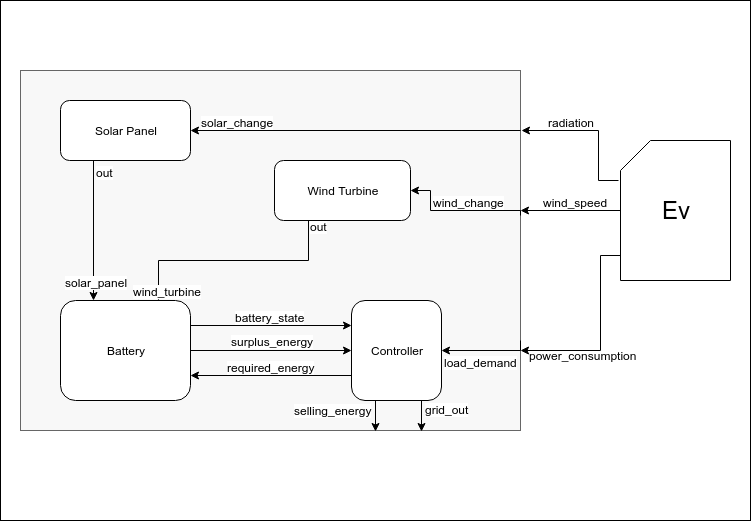
\includegraphics[scale=0.5]{images/casa.png}
    \caption{Diagrama con la descripción del \textit{top model} simulado.}
\end{figure}